\section{Nummerical Simulation}
\begin{figure}[H]
    \centering
    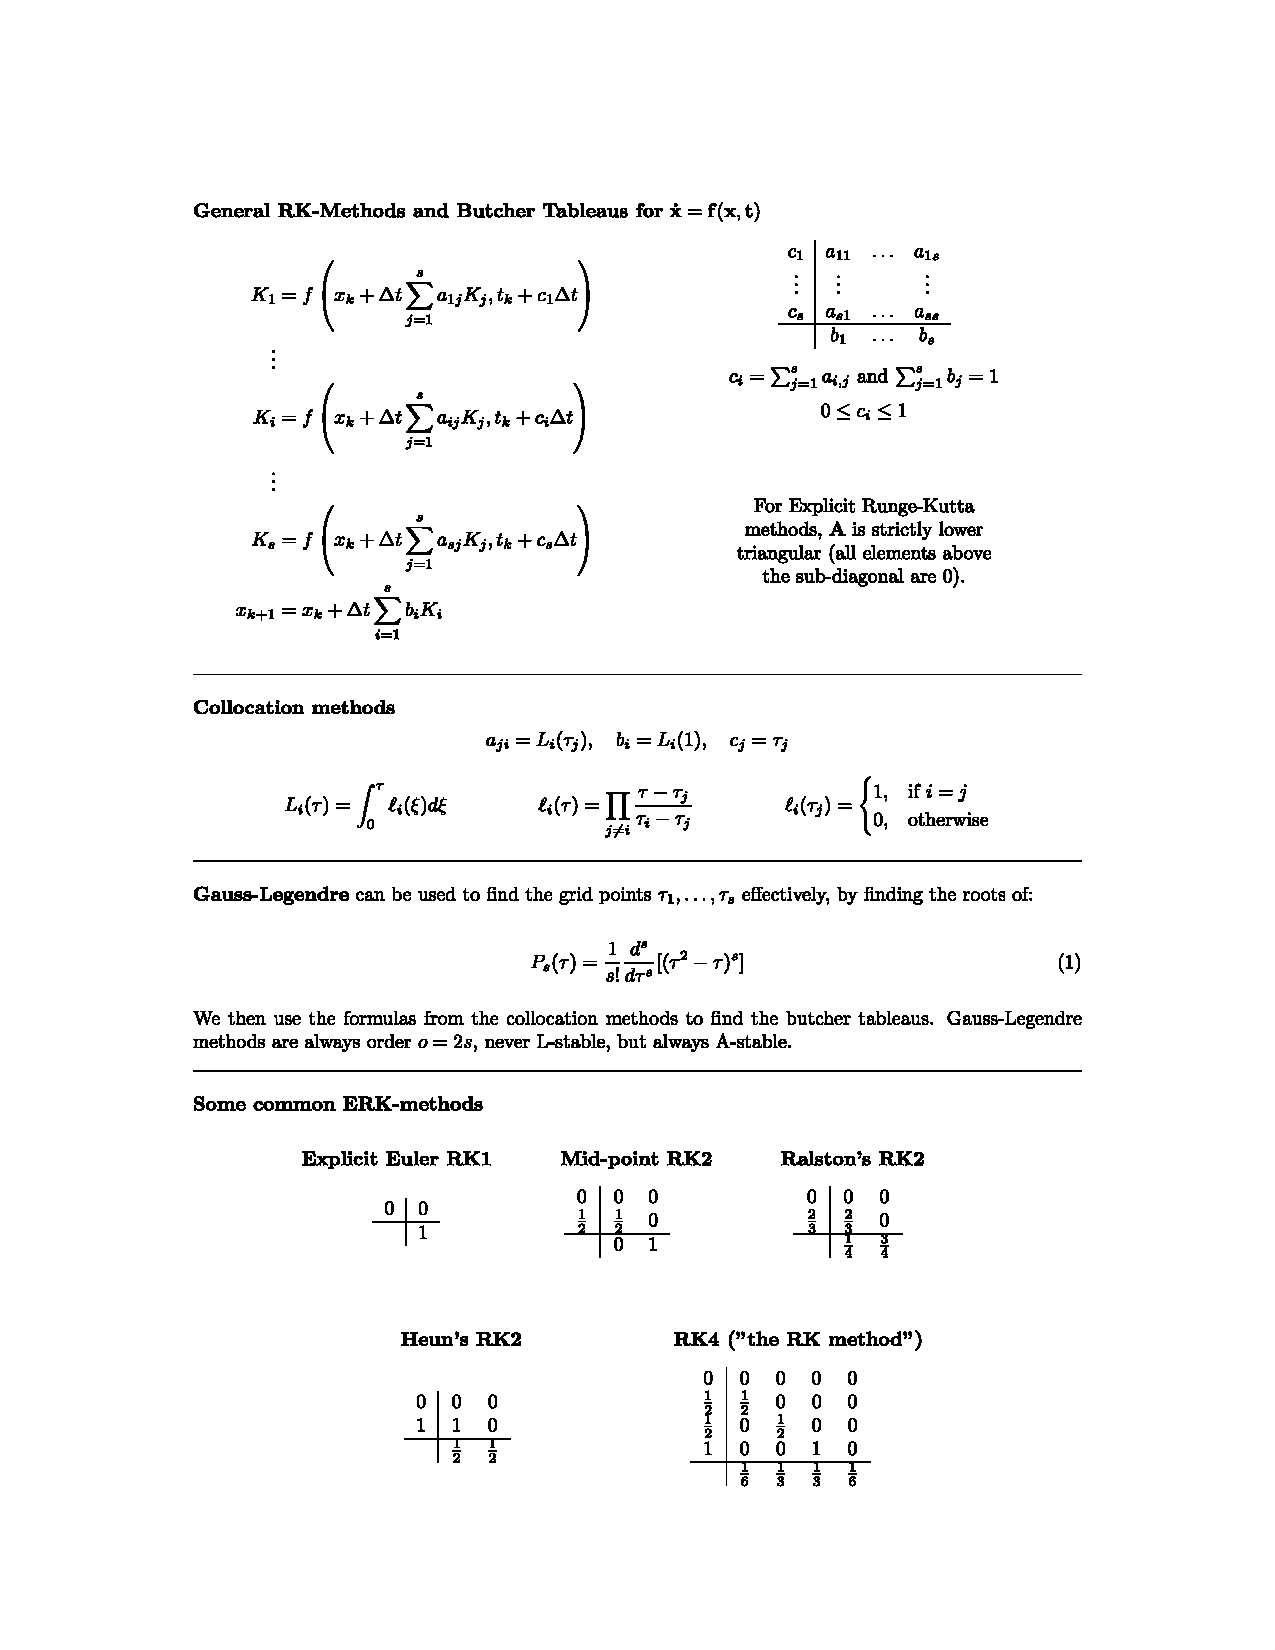
\includepdf[width=\linewidth]{figures/sim1.pdf}
\end{figure}
\newpage
\begin{figure}[H]
    \centering
    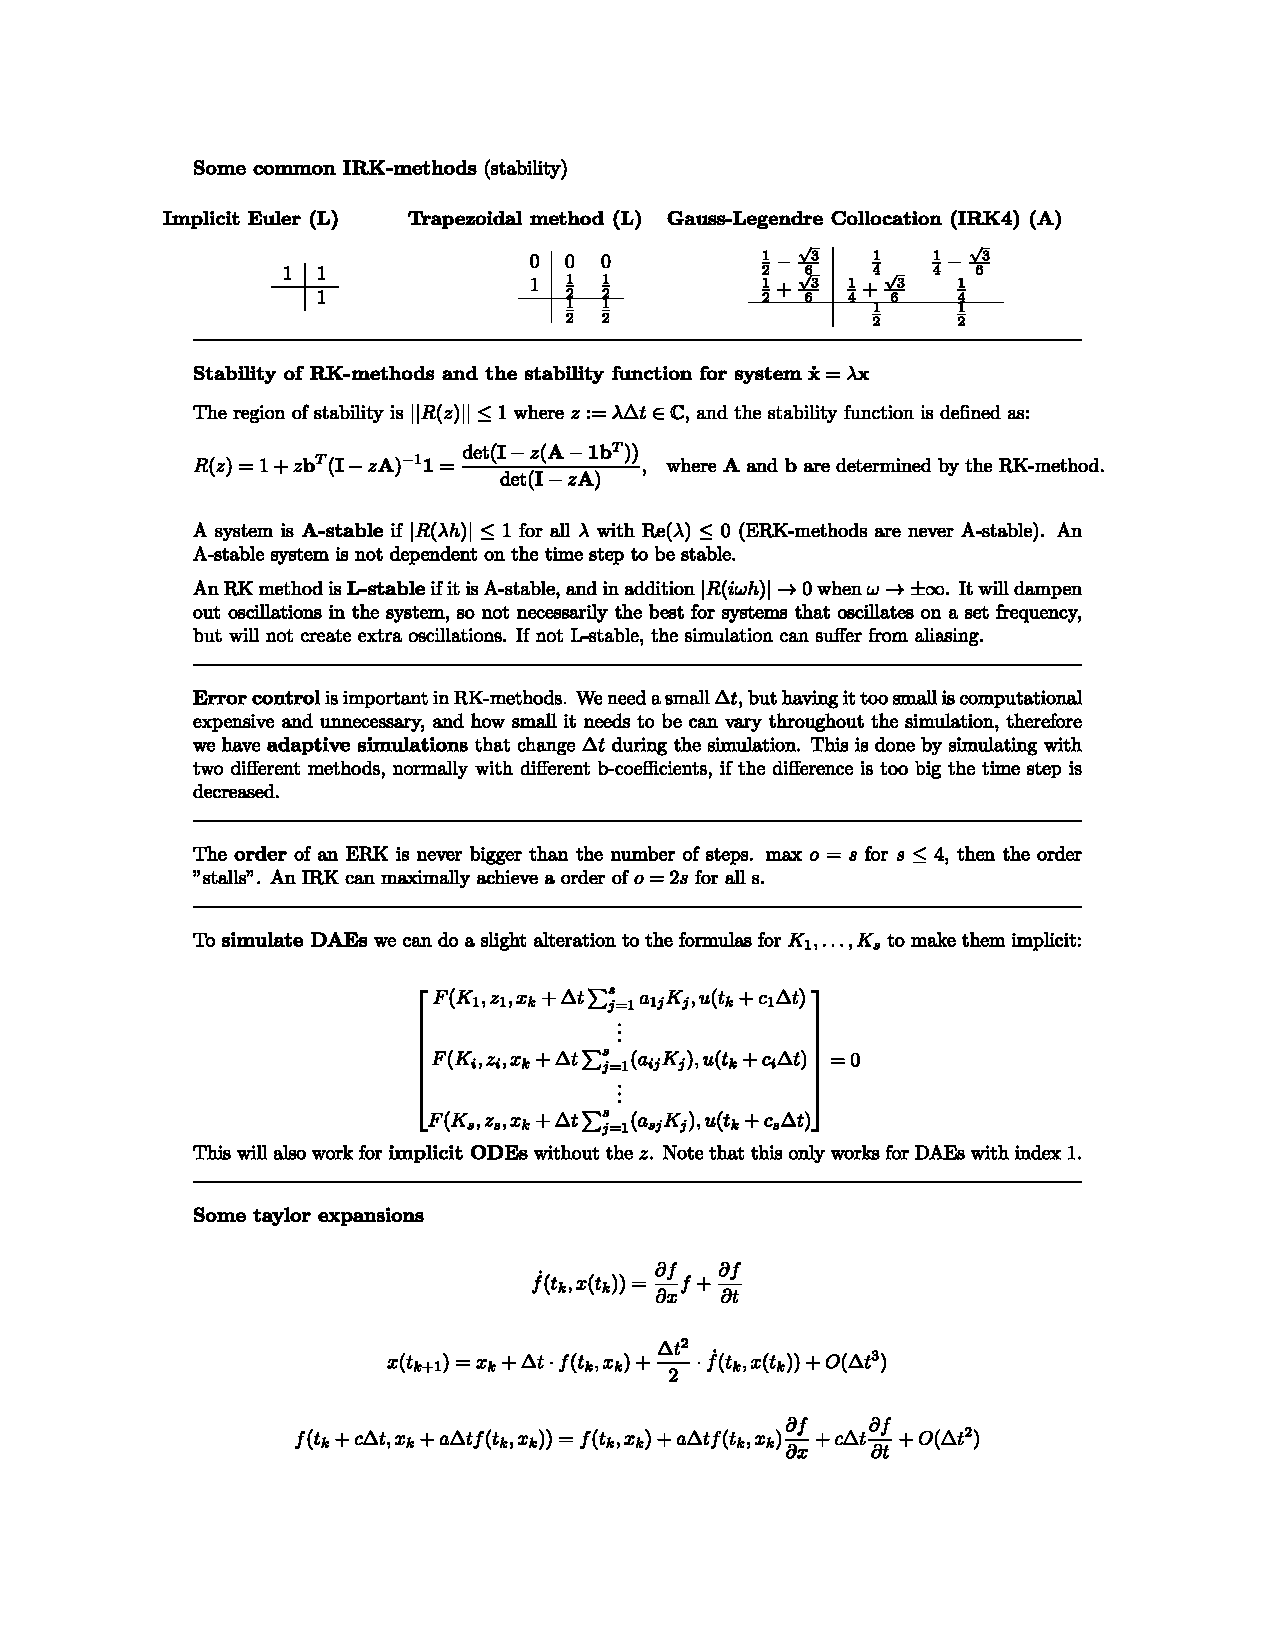
\includepdf[width=\linewidth]{figures/sim2.pdf}
\end{figure}
\newpage


\subsection{Explicit }

\textbf{The Forward Euler method}
\begin{subequations}
\begin{align}
    x_{k+1} = x_k + \Delta t \cdot f(x_k)\\
    x_n = n \cdot \Delta t \cdot v \label{eq:Euler}
\end{align}
\end{subequations}

This method is first order, which means global error E is proportional to step size h. 

Stable for: \[\Delta t < - \frac{2}{\lambda}\]

\textbf{Runke gutta 2: Mid Point Method }

Want to evaluate \(\dot{x} = f(x)\) between \(t_k\) and \(t_{k+1}\) (omitting \(u\) and \(t\) for ease of notation):
\begin{equation}
x_{k+1} = x_k + \Delta t f\left( x \left( t_k + \frac{1}{2} \Delta t \right) \right)
\end{equation}

\textbf{Euler Half-Step}
Need to estimate \(x \left( t_k + \frac{1}{2} \Delta t \right)\):
\begin{equation}
x \left( t_k + \frac{1}{2} \Delta t \right) \approx x_k + \frac{1}{2} \Delta t f(x_k)
\end{equation}

The Mid-point Method can also be formulated as:

\begin{align}
k_1 &= f(x_k) \\
k_2 &= f\left(x_k + \frac{1}{2} \Delta t k_1\right) \\
x_{k+1} &= x_k + \Delta t k_2
\end{align}

The Mid-point method is second order.  This means the global error E is proportional to the square of the step size h.
\\
\\
The stability criterion is given by:
\begin{equation}
\left| 1 + \Delta t \lambda + \frac{(\Delta t \lambda)^2}{2} \right| \leq 1
\end{equation}

\textbf{4tho-Order runke gutta }

\begin{align}
k_1 &= f(t_n, x_n) \\
k_2 &= f\left(t_n + \frac{h}{2}, x_n + \frac{h}{2} k_1\right) \\
k_3 &= f\left(t_n + \frac{h}{2}, x_n + \frac{h}{2} k_2\right) \\
k_4 &= f(t_n + h, x_n + h k_3) \\
x_{n+1} &= x_n + \frac{h}{6} \left( k_1 + 2k_2 + 2k_3 + k_4 \right)
\end{align}

The Butcher tableau for the RK4 method is:

\[
\begin{array}{c|cccc}
0 & 0 & 0 & 0 & 0 \\
\frac{1}{2} & \frac{1}{2} & 0 & 0 & 0 \\
\frac{1}{2} & 0 & \frac{1}{2} & 0 & 0 \\
1 & 0 & 0 & 1 & 0 \\
\hline
 & \frac{1}{6} & \frac{1}{3} & \frac{1}{3} & \frac{1}{6} \\
\end{array}
\]
\\
\\
if stiff use implicit runke gutta aahhhh


\subsection{Implecit Runke gutta}
\textbf{A- stability}
\\
\\
A numerical method is said to be A-stable if for any \(\lambda\) with \(\text{Re}(\lambda) \leq 0\), the stability function \(R(z)\) of the method satisfies:

\[
|R(\Delta t \lambda)| \leq 1
\]

for all step sizes \(\Delta t\). where  $|R(\Delta t \lambda)$ is the stabilityf function with the eigenvalues $\lambda$  of the jacobian (usikker om dette), only IRK can be A-stable.